% --------------------------------------
% Document Class
% --------------------------------------
\documentclass[a4paper,11pt]{article}
% --------------------------------------



% --------------------------------------
% Use Package
% --------------------------------------


\usepackage[francais]{babel}
%\usepackage{ucs}
\usepackage[utf8]{inputenc}
\usepackage[T1]{fontenc}

\usepackage{makeidx}
\usepackage{color}
\usepackage{graphicx}
\usepackage{float}
\usepackage[hidelinks]{hyperref} 
\usepackage{geometry}
%\usepackage{lastpage}
%\usepackage{marginnote}
\usepackage{fancyhdr}
%\usepackage{titlesec}
%\usepackage{framed}
\usepackage{amsmath}
\usepackage{empheq}
\usepackage{array}
\usepackage{multicol}
\usepackage{csquotes}
%\usepackage{adjustbox}

% insert code
\usepackage{listings}

% define our color
\usepackage{xcolor}

% code color
\definecolor{ligthyellow}{RGB}{250,247,220}
\definecolor{darkblue}{RGB}{5,10,85}
\definecolor{ligthblue}{RGB}{1,147,128}
\definecolor{darkgreen}{RGB}{8,120,51}
\definecolor{darkred}{RGB}{160,0,0}

% other color
\definecolor{ivi}{RGB}{141,107,185}


\lstset{
    language=java,
    captionpos=b,
    extendedchars=true,
    frame=lines,
    numbers=left,
    numberstyle=\tiny,
    numbersep=5pt,
    keepspaces=true,
    breaklines=true,
    showspaces=false,
    showstringspaces=false,
    breakatwhitespace=false,
    stepnumber=1,
    showtabs=false,
    tabsize=3,
    basicstyle=\small\ttfamily,
    backgroundcolor=\color{ligthyellow},
    keywordstyle=\color{ligthblue},
    morekeywords={include, printf, uchar},
    identifierstyle=\color{darkblue},
    commentstyle=\color{darkgreen},
    stringstyle=\color{darkred},
}


% --------------------------------------



% --------------------------------------
% Page setting
% --------------------------------------
%\pagestyle{empty}
\setlength{\headheight}{15pt}

\setcounter{secnumdepth}{3}
\setcounter{tocdepth}{2}

\makeatletter
\@addtoreset{chapter}{part}
\makeatother 

\hypersetup{         % parametrage des hyperliens
  colorlinks=true,      % colorise les liens
  breaklinks=true,      % permet les retours à la ligne pour les liens trop longs
  urlcolor= blue,       % couleur des hyperliens
  linkcolor= black,     % couleur des liens internes aux documents (index, figures, tableaux, equations,...)
  citecolor= green      % couleur des liens vers les references bibliographiques
}

% --------------------------------------

% --------------------------------------
% Information
% --------------------------------------
\title{Compte-rendu TP11 TI : Formation des images couleur et dématriçage}
\author{Elliot VANEGUE et Gaëtan DEFLANDRE}
% --------------------------------------

\definecolor{myColor}{rgb}{0.5, 0.1, 0.75}

% --------------------------------------
% Begin content
% --------------------------------------
\begin{document}

% Set language to english
  \selectlanguage{francais}

  % Start the page counting
  \pagenumbering{arabic}

  \maketitle
  
  \mbox{}
  \newpage
  \clearpage
  
  \section{Introduction}
  Avant de pouvoir traiter une image, il faut pouvoir l'acquérir au moyen de capteur présent dans les
  caméra ou appareil photo par exemple. Dans nos appareils grand public, un capteur est composé d'une mosaîque
  de pixel. Les pixels ne peuvent représenter qu'un seul dégradé de couleur. C'est pourquoi il existe différent
  CFA\footnote{Color Filter Array} qui permettent d'obtenir une image couleur. Durant ce TP, nous allons voir
  comment est utilisé le CFA de Bayer.
  
  \section{Interprétation et simulation d'une image CFA}
  Etant donné que nous travaillons sur une image acquise avec un CFA de Bayer, nous pouvons déterminer quelle est
  la disposition des pixels de l'image. Lorsque nous regardons le coin haut gauche, qui représente un ciel bleu, nous
  constatons que le troisième pixel est plus claire que les deux premiers dans l'image CFA. Or le troisième pixel 
  a une valeur dans la composante bleu qui est plus importante que les deux premiers pixels. Donc la première configuration
  de Bayer utilisé sur notre image est la suivante : \\
  
  \begin{figure}[H]
  \center
   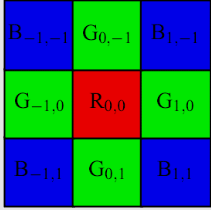
\includegraphics[width=3cm]{bayerGRG.png}
  \end{figure}

  Nous allons maintenant simuler la génération d'une image CFA à partir de l'image couleur. Pour
  cela nous appelons la méthode \enquote{cfa} qui nous est fournit et nous stockons le résultat
  dans un ImageProcessor que nous affichons. Nous obtenons ainsi une image CFA dont la configuration
  est la suivante :
  
  \begin{figure}[H]
  \center
   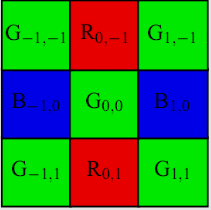
\includegraphics[width=3cm]{bayerBGB.png}
  \end{figure}
  
  Nous obtenons donc une image en dégradé de gris, car une image CFA ne comporte qu'un seul canal par pixel,
  c'est après un dématriçage que l'image possèdera trois canaux représentant chaque composante couleur.
  
  \section{Dématriçage par interpolation bilinéaire}
  Nous avons dans notre cours les quatre formules de dématriçage suivante :
  
  \begin{align}
  B = \frac{1}{4} * (B_{-1,-1}+B_{1,-1}+B_{-1,1}+B_{1,1})\\
  G = \frac{1}{4} * (G_{0,-1}+G_{-1,0}+G_{1,0}+G_{0,1})\\
  R = \frac{1}{2} * (R_{-1,0}+R_{1,0})\\
  B = \frac{1}{2} * (B_{0,-1}+B_{0,1})
  \end{align}
  
  Cela nous permet dans un premier temps de définir le masque de la composante G $\frac{1}{4}$
  $\begin{pmatrix}
   0 & 1 & 0\\
   1 & 4 & 1\\
   0 & 1 & 0
  \end{pmatrix}$
  puisque l'on peut voir dans l'équation de G qu'il a besoin de ses voisins du dessus, du dessous,
  de gauche et de droite afin de calculer le pixel courant. Pour les composantes suivantes, le calcul
  est un peu plus complexe, car leur équation varie en fonction de la configuration du CFA. Le masque
  correspondant aux deux autres composantes est $\frac{1}{4}$
  $\begin{pmatrix}
   1 & 2 & 1\\
   2 & 4 & 2\\
   1 & 2 & 1
  \end{pmatrix}$. Dans cette matrice, les valeurs en (1,0), (0,1), (-1,0) et (0,-1) sont à 2, car 
  les équations 3 et 4 ont un coefficient non pas de $\frac{1}{4}$ mais de $\frac{1}{2}$, il faut
  donc leur donner un poid deux plus important que le reste des voisins. Le reste des voisins n'ont 
  qu'un poid de 1 dans le masque grâce à l'équation 1.
  
  %TODO probleme sur la macro -> mauvais resultat mais le plug in fait le bon truc
  
  \section{Dématriçage basé sur l'estimation locale d'un gradient}
  
 
  %TODO pas oublier de mettre le code
\end{document}  